\chapter{Desarrollo de las prácticas}
\label{chap:desarrollo}

\lettrine{E}{n} este capítulo se describe detalladamente el trabajo realizado durante las prácticas, organizando las actividades cronológicamente y destacando los principales hitos, retos y aprendizajes.

\section{Primera etapa: Configuración y familiarización}
\label{sec:primera_etapa}

Durante la primera semana, el enfoque principal fue la configuración del entorno y la familiarización con las herramientas y flujos de trabajo de la empresa. Las actividades incluyeron:

\begin{itemize}
    \item \textbf{Presentación y configuración inicial:} Reunión con recursos humanos, entrega de equipos, claves y lectura de documentos sobre protección de datos y flujos de trabajo.
    \item \textbf{Configuración del entorno de desarrollo:} Instalación de herramientas clave como DVC, Conda, Python, Docker, Visual Studio Code con extensiones específicas (gitlens, c/c++, Python), y configuraciones para proyectos con CMake y Make.
    \item \textbf{Familiarización con las plataformas de gestión:} Estudio de herramientas internas como MLflow, CVAT y DVC, utilizadas para gestionar experimentos, etiquetado y datasets.
    \item \textbf{Primeras pruebas prácticas:} Subida y etiquetado de videos en CVAT, identificando retos como la latencia en el etiquetado de objetos móviles (ej., pelotas).
\end{itemize}

\section{Segunda etapa: Mejoras en detección de marcadores}
\label{sec:segunda_etapa}

El objetivo de esta etapa fue optimizar el sistema de detección de marcadores deportivos. Entre las actividades más relevantes destacan:

\subsection{Detección de marcadores apagados}
\label{subsec:marcadores_apagados}

Se implementaron mejoras en la detección de marcadores con bajo contraste o apagados:

\begin{itemize}
    \item \textbf{Generación de datasets específicos:} Captura y etiquetado de imágenes de marcadores en condiciones adversas.
    \item \textbf{Actualización del diccionario:} Inclusión de caracteres adicionales como espacios y símbolos necesarios para nuevos escenarios.
    \item \textbf{Reentrenamiento de modelos:} Entrenamientos iterativos con los nuevos datos para mejorar la precisión de las detecciones.
\end{itemize}

Estas mejoras se reflejaron en las métricas de Word Error Rate (WER), reduciendo el error global del 23.4\% al 18.7\% (ver Tabla \ref{tab:metricas}).

\begin{table}[h]
\centering
\begin{tabular}{|l|c|c|}
\hline
\textbf{Métrica} & \textbf{Antes} & \textbf{Después} \\
\hline
Global WER & 0.234 & 0.187 \\
\hline
\end{tabular}
\caption{Mejora en métricas de detección}
\label{tab:metricas}
\end{table}

\section{Tercera etapa: Investigación en TTS}
\label{sec:tercera_etapa}

Durante esta fase, se exploraron tecnologías de síntesis de voz, evaluando múltiples modelos y realizando pruebas exhaustivas.

\subsection{Modelos evaluados}
\label{subsec:tts_modelos}
Entre los modelos analizados, se incluyen:

\begin{itemize}
    \item \textbf{Coqui TTS:} Plataforma versátil que integra modelos como XTTSv2 (clonación de voz), Tacotron2 con HiFi-GAN (síntesis natural) y VITS.
    \item \textbf{OpenVoice v2:} Sistema TTS enfocado en personalización y soporte multilingüe.
    \item \textbf{IMS-Toucan:} Modelo que destaca por su adaptabilidad y cantidad de idiomas soportados (aunque no todos tienen la misma calidad de síntesis).
    \item \textbf{Mozilla TTS:} Herramienta extensible para la creación de modelos personalizados.
\end{itemize}

\begin{figure}[h]
    \centering
    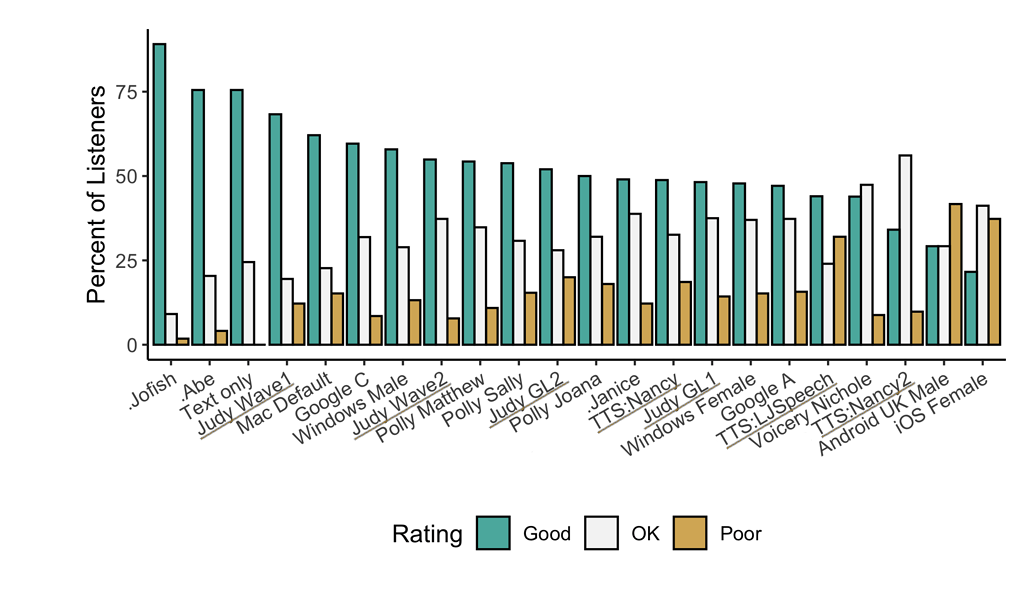
\includegraphics[width=0.8\textwidth]{04_imaxes/TTS-performance.png}
    \caption{Desempeño de modelos disponibles en Coqui TTS}
    \label{fig:tts_performance}
\end{figure}

\subsection{Fine-tuning de modelos}
\label{subsec:tts_fine_tuning}
Se realizaron ajustes finos en modelos seleccionados, siguiendo estos pasos:

\begin{itemize}
    \item \textbf{Creación de datasets:} Generación y normalización de datos de entrenamiento utilizando herramientas como Whisper y ffmpeg.
    \item \textbf{Ajustes de parámetros:} Pruebas con configuraciones avanzadas para mejorar la calidad de la síntesis.
    \item \textbf{Evaluación:} Comparación de métricas para identificar el impacto de las mejoras.
\end{itemize}

\section{Herramientas y tecnologías utilizadas}
\label{sec:herramientas}

Durante las prácticas se emplearon diversas herramientas tecnológicas, entre las que destacan:

\begin{itemize}
    \item \textbf{Control de versiones:} Git y GitLab para la gestión del código.
    \item \textbf{ML/CV:} Herramientas como MLflow, DVC y CVAT para gestionar experimentos y datasets.
    \item \textbf{Contenedores:} Docker y docker-compose para contenerización.
    \item \textbf{CI/CD:} GitLab CI y pre-commit para automatizar flujos de trabajo.
    \item \textbf{Audio/Video:} ffmpeg y Whisper para procesamiento y transcripción.
    \item \textbf{Otros:} Python, bash y tmux para tareas diversas.
\end{itemize}

\section{Retos y soluciones}
\label{sec:retos}

A lo largo de las prácticas se enfrentaron diversos desafíos, entre ellos:

\begin{itemize}
    \item \textbf{Gestión de dependencias:} Resuelto mediante el uso de entornos virtuales y Docker.
    \item \textbf{Limitaciones de hardware:} Optimización de parámetros y uso de máquinas remotas con GPUs de alta capacidad.
    \item \textbf{Problemas de inferencia:} Mejora de datasets y reentrenamiento de modelos para corregir errores específicos.
    \item \textbf{Procesos zombie:} Uso de tmux para una gestión robusta de sesiones.
\end{itemize}